
%%%%%%%%%%%%%%%%%%%%%%% file typeinst.tex %%%%%%%%%%%%%%%%%%%%%%%%%
%
% This is the LaTeX source for the instructions to authors using
% the LaTeX document class 'llncs.cls' for contributions to
% the Lecture Notes in Computer Sciences series.
% http://www.springer.com/lncs       Springer Heidelberg 2006/05/04
%
% It may be used as a template for your own input - copy it
% to a new file with a new name and use it as the basis
% for your article.
%
% NB: the document class 'llncs' has its own and detailed documentation, see
% ftp://ftp.springer.de/data/pubftp/pub/tex/latex/llncs/latex2e/llncsdoc.pdf
%
%%%%%%%%%%%%%%%%%%%%%%%%%%%%%%%%%%%%%%%%%%%%%%%%%%%%%%%%%%%%%%%%%%%


\documentclass[runningheads,a4paper]{llncs}

\usepackage{amssymb}
\setcounter{tocdepth}{3}
\usepackage{graphicx}
%\usepackage{listings}

\usepackage{url}
\urldef{\mailsa}\path|{alfred.hofmann, ursula.barth, ingrid.haas, frank.holzwarth,|
\urldef{\mailsb}\path|anna.kramer, leonie.kunz, christine.reiss, nicole.sator,|
\urldef{\mailsc}\path|erika.siebert-cole, peter.strasser, lncs}@springer.com|    
\newcommand{\keywords}[1]{\par\addvspace\baselineskip
\noindent\keywordname\enspace\ignorespaces#1}

\begin{document}

\mainmatter  % start of an individual contribution

% first the title is needed
\title{Semantic Annotation Semantically: Using a~Shareable Extraction Ontology and a Reasoner}

% a short form should be given in case it is too long for the running head
\titlerunning{Semantic Annotation Semantically}

% the name(s) of the author(s) follow(s) next
%
% NB: Chinese authors should write their first names(s) in front of
% their surnames. This ensures that the names appear correctly in
% the running heads and the author index.
%
\author{Jan D\v{e}dek \and Peter Vojt\'{a}\v{s}}
%\thanks{Please note that the LNCS Editorial assumes that all authors have used
%the western naming convention, with given names preceding surnames. This determines
%the structure of the names in the running heads and the author index.}%
%
\authorrunning{Jan D\v{e}dek \and Peter Vojt\'{a}\v{s}}
% (feature abused for this document to repeat the title also on left hand pages)

% the affiliations are given next; don't give your e-mail address
% unless you accept that it will be published
\institute{Department of Software Engineering, Charles University,\\
Prague, Czech Republic
\\\url{{dedek,vojtas}@ksi.mff.cuni.cz}}

%
% NB: a more complex sample for affiliations and the mapping to the
% corresponding authors can be found in the file "llncs.dem"
% (search for the string "\mainmatter" where a contribution starts).
% "llncs.dem" accompanies the document class "llncs.cls".
%

%\toctitle{Semantic Annotation Semantically: Using a Shareable Extraction Ontology and a Reasoner}
%\tocauthor{Jan D\v{e}dek and Peter Vojt\'{a}\v{s}}
\maketitle


\begin{abstract}
In this paper we present a method for semantic annotation of texts, which is based on a deep linguistic analysis (DLA) and Inductive Logic Programming xxxxxxxxxxxxxxxxxxxxxxxx

A description, implementation and initial evaluation of the method are the main contributions of the paper.
\keywords{Semantic Annotation, Dependency Linguistics, Inductive Logic Programming, Information Extraction, Machine Learning}
\end{abstract}


%%%%%%%%%%%%%%%%%%%%%%%%%%%%%%%%%%%%%%%%%%%%%%%%%%%%%%%%%%%%%%%%%%%%%%%%%%%%%%%%%%%%%%%%%%%%%%%%%%%%%%%%%%%%%%
\section{Introduction}
%%%%%%%%%%%%%%%%%%%%%%%%%%%%%%%%%%%%%%%%%%%%%%%%%%%%%%%%%%%%%%%%%%%%%%%%%%%%%%%%%%%%%%%%%%%%%%%%%%%%%%%%%%%%%%


Information extraction (IE) and automated semantic annotation of text are usually done by complex tools and all these tools use some kind of a model that represents the actual task and its solution. The model is usually represented as a set of some kind of extraction rules (e.g. regular expressions), gazetteer lists or it is based on some statistical measurements and probability assertions (classification algorithms like Support Vector Machines (SVM), Maximum Entropy Models, Decision Trees, Hidden Markov Models (HMM), Conditional Random Fields (CRF), etc.)

In the begging a model is either created by a human user or it is learned from a training dataset. Then, in an actual extraction/annotation process, the model is used as a configuration or as an input parameter of the particular extraction/annotation tool. These models are usually stored in proprietary formats and they are accessible only by the corresponding tool.

In the environment of the Semantic Web it is essential that information is sharable and some ontology based IE tools keep the model in so called extraction ontologies. Extraction ontologies should serve as a wrapper for documents of a narrow domain of interest. When we apply an extraction ontology to a document, the ontology identifies objects and relationships present in the document and it associates them with the corresponding ontology terms and thus wraps the document so that it is understandable in terms of the ontology \cite{DBLP:conf/er/EmbleyTL02}.



In practice the extraction ontologies are usually strongly dependent on a particular extraction/annotation tool and cannot be used separately. The strong dependency of an extraction ontology on the corresponding tool makes it very difficult to share. When an extraction ontology cannot be used outside the tool there is also no need to keep the ontology in a standard ontology format such as RDF\footnote{\url{http://www.w3.org/RDF/}} or OWL\footnote{\url{http://www.w3.org/2001/sw/wiki/OWL}}. The only possibility how to use such extraction ontology is within the corresponding extraction tool. It is not necessary to have the ontology in a `owl' or `rdf' file. In a sense such extraction ontology is just a configuration file. For example in \cite{springerlink:10.1007/978-3-642-01891-6_5} %[Labsky]
 (and also in \cite{DBLP:conf/er/EmbleyTL02}) the so called extraction ontologies are kept in XML files with a proprietary structure and it is absolutely sufficient, there is no need to treat them differently.


\subsection{Shareable Extraction Ontologies}

In this paper we present an extension of the idea of extraction ontologies. We adopt the point that extraction models are kept in extraction ontologies and we add that the extraction ontologies should not be dependent on the particular extraction/annotation tool. In such case the extraction/annotation process can be done separately by an ordinary reasoner.


In this paper we present a proof of a concept for the idea: a case study with our linguistically based IE engine and an experiment with several OWL reasoners. In the case study (see Section~\ref{sec:case}) the IE engine exports its extraction rules to the form of an extraction ontology. Third party linguistic tool linguistically annotates an input document and the linguistic annotations are translated to so-called document ontology. After that an ordinary OWL reasoner is used to apply the extraction ontology on the document ontology, which has the same effect as a direct application of the extraction rules on the document.
In Section~\ref{sec:experiment} we present an experiment with several OWL reasoner and IE datasets to verify feasibility of the idea.  





%%%%%%%%%%%%%%%%%%%%%%%%%%%%%%%%%%%%%%%%%%%%%%%%%%%%%%%%%%%%%%%%%%%%%%%%%%%%%%%%%%%%%%%%%%%%%%%%%%%%%%%%%%%%%%
\section{Related Work}
%%%%%%%%%%%%%%%%%%%%%%%%%%%%%%%%%%%%%%%%%%%%%%%%%%%%%%%%%%%%%%%%%%%%%%%%%%%%%%%%%%%%%%%%%%%%%%%%%%%%%%%%%%%%%%
Ontology-based Information Extraction (OBIE) \cite{citeulike:7291004} or Ontology-driven Information Extraction \cite{Yildiz:2007:OMO:1793154.1793216} has recently emerged as a subfield of information extraction. Also Web Information Extraction \cite{DBLP:journals/tkde/ChangKGS06} is a closely related discipline. Many extraction and annotation tools can be found in the above mentioned surveys \cite{citeulike:7291004,DBLP:journals/tkde/ChangKGS06} and many of the tools also use an ontology as an output format, but almost all of them store their extraction models in proprietary formats and the models are accessible only by the corresponding tool.

In the literature we have found only two approaches that use extraction ontologies. The former one was published by D. Embley \cite{DBLP:conf/er/EmbleyTL02,Embley:2004:TSU:1012294.1012295}
and the later one IE system Ex \footnote{\url{http://eso.vse.cz/~labsky/ex/}} published by M. Labsk\'{y} \cite{springerlink:10.1007/978-3-642-01891-6_5}. 
But in both cases the extraction ontologies are dependent on the particular tool and they are kept in XML files with a proprietary structure.


Also authors of \cite{citeulike:7291004} (a recent survey of OBIE systems) do not agree with allowing for extraction rules to be a part of an ontology. They use two arguments against that:
\begin{enumerate}
	\item Extraction rules are known to contain errors (because they are never 100\% accurate), and objections can be raised on their inclusion in ontologies in terms of formality and accuracy.

	\item It is hard to argue that linguistic extraction rules should be considered a part of an ontology while information extractors based on other IE techniques (such as SVM, HMM, CRF, etc. classifiers used to identify instances of a class when classification is used as the IE technique) should be kept out of it: all IE techniques perform the same task with comparable effectiveness (generally successful but not 100\% accurate). But the techniques advocated for the inclusion of linguistic rules in ontologies cannot accommodate such IE techniques. They assert that either all information extractors (that use different IE techniques) should be included in the ontologies or none should be included.
\end{enumerate}



Concerning the first argument, we have to take into account that extraction ontologies are not ordinary ontologies, it should be agreed that they do not contain 100\% accurate knowledge. Also the estimated accuracy of the extraction rules can be saved in the extraction ontology and it can then help potential users to decide how much they will trust the extraction ontology.

Concerning the second argument, we agree that it is not always possible to save an extraction model to an ontology. But on the other hand we think that there are cases when shareable extraction ontologies can be useful. And maybe in the future; if this idea proves its usefulness; new standard ways how to encode models to an ontology will appear.


Also the most widely agreed definitions of an ontology emphasize the shared aspect of ontologies. 
\begin{quote}
An ontology is a formal specification of a shared conceptualization.	\cite{so17864}
\end{quote}

\begin{quote}
An ontology is a formal, explicit specification of a shared conceptualization. \cite{Studer1998161}
\end{quote}

Of course the word `sharable' has different meaning form `shared'. Something that is shareable is not necessarily shared, but on the other hand something that is shared should be shareable. We do not think that shareable extraction ontologies will contain shared knowledge about how to extract data form documents in certain domain. This is for example not true for all extraction models artificially leaned from a training corpus. Here shareable simply means that the extraction rules can be shred amongst software agents and can be used separately form the original tool. In time it will turn out if such extraction ontologies are useful or not. But for sure they bring something new that was not possible before.




%%%%%%%%%%%%%%%%%%%%%%%%%%%%%%%%%%%%%%%%%%%%%%%%%%%%%%%%%%%%%%%%%%%%%%%%%%%%%%%%%%%%%%%%%%%%%%%%%%%%%%%%%%%%%%
\section{The Main Idea Illustrated -- Our Case Study} \label{sec:case}
%%%%%%%%%%%%%%%%%%%%%%%%%%%%%%%%%%%%%%%%%%%%%%%%%%%%%%%%%%%%%%%%%%%%%%%%%%%%%%%%%%%%%%%%%%%%%%%%%%%%%%%%%%%%%%

In this section we will describe the main idea of the paper and we will illustrate it with a case study.

\subsection{Document Ontologies} \label{sec:doc_ont}

The main idea of this paper assumes that extraction ontologies will be shareable and they can be applied on a document outside of the original extraction/annotation tool. We further assume that the extraction ontologies will be applied by ordinary reasoners. This assumption implies that both extraction ontologies and documents have to be in a reasoner readable format. In the case of contemporary OWL reasoners there are standard reasoner-readable languages: OWL and RDF in a rich variety of possible serializations like ((RDF/OWL)-XML, Turtle, N-Triples, etc.) Besides that there exists standard ways like GRDDL\footnote{\url{http://www.w3.org/TR/grddl/}} or RDFa\footnote{\url{http://www.w3.org/TR/xhtml-rdfa-primer/}} how to transform an ordinary document to a RDF document. We call the output of such transformation a `document ontology'. A document ontology should contain all relevant data of a document and preferably the document could be reconstructed from the document ontology on demand.

When a reasoner is applying an extraction ontology to a document, it has only ``to annotate'' the corresponding document ontology. Here ``to annotate'' means to add new knowledge -- new class membership or property assertions. In fact it means just to do the inference tasks prescribed by the extraction ontology on the document ontology. 


\subsection{Implementation}

In this section we will present details abut the case study.  We have used our IE engine \cite{biblio:DedekISWC2010} based on deep linguistic parsing and Inductive Logic Programming. It is a complex system implemented with a great help of the GATE system\footnote{\url{http://gate.ac.uk/}} \cite{dedek:GATE_ACL2002} and it also uses many other third party tools including several linguistic tools a Prolog system. Installation and making the system operate is not simple. This case study should demonstrate that the extraction rules produced by the system are not dependent on the system in the sense described above.




\subsubsection{Linguistic Analysis}

Our IE engine needs a linguistic preprocessing (deep linguistic parsing) of documents on its input. Deep linguistic parsing brings a very complex structure to the text and the structure serves as a footing for construction and application of extraction rules. 

We usually use TectoMT system\footnote{\url{http://ufal.mff.cuni.cz/tectomt/}} \cite{dedek:ZaPtTectoMTHighly2008} to do the linguistic preprocessing. TectoMT is a Czech project that contains many linguistic analyzers for different languages including Czech and English. We are using a majority of applicable tools from TectoMT: a tokeniser, a sentence splitter, morphological analyzers (including POS tagger), a syntactic parser and the deep syntactic (tectogrammatical) parser. All the tools are based on the dependency based linguistic theory and formalism of the Prague Dependency Treebank project \footnote{\url{http://ufal.mff.cuni.cz/pdt2.0/}} \cite{dedek:PDT20_CD}.

The output linguistic annotations of the TectoMT system are stored (along with the text of the source document) in XML files in so called Prague Markup Language\footnote{\url{http://ufal.mff.cuni.cz/jazz/PML/}} (PML). PML is a very complex language (or XML schema) that is able to express many linguistic elements and features present in text. For the IE engine a tree dependency structure of words in sentences is the most useful one because the edges of the structure guide the extraction rules. An example of such (tectogrammatical) tree structure is in Fig.~\ref{img:tree}.

In this case study PML files made form source documents by TectoMT are transformed to RDF document ontology by a quite simple GRDDL/XSLT\footnote{\url{http://www.w3.org/TR/xslt}} transformation. Such document ontology contains the whole variety of PML in RDF format.





\begin{figure}
\centerline{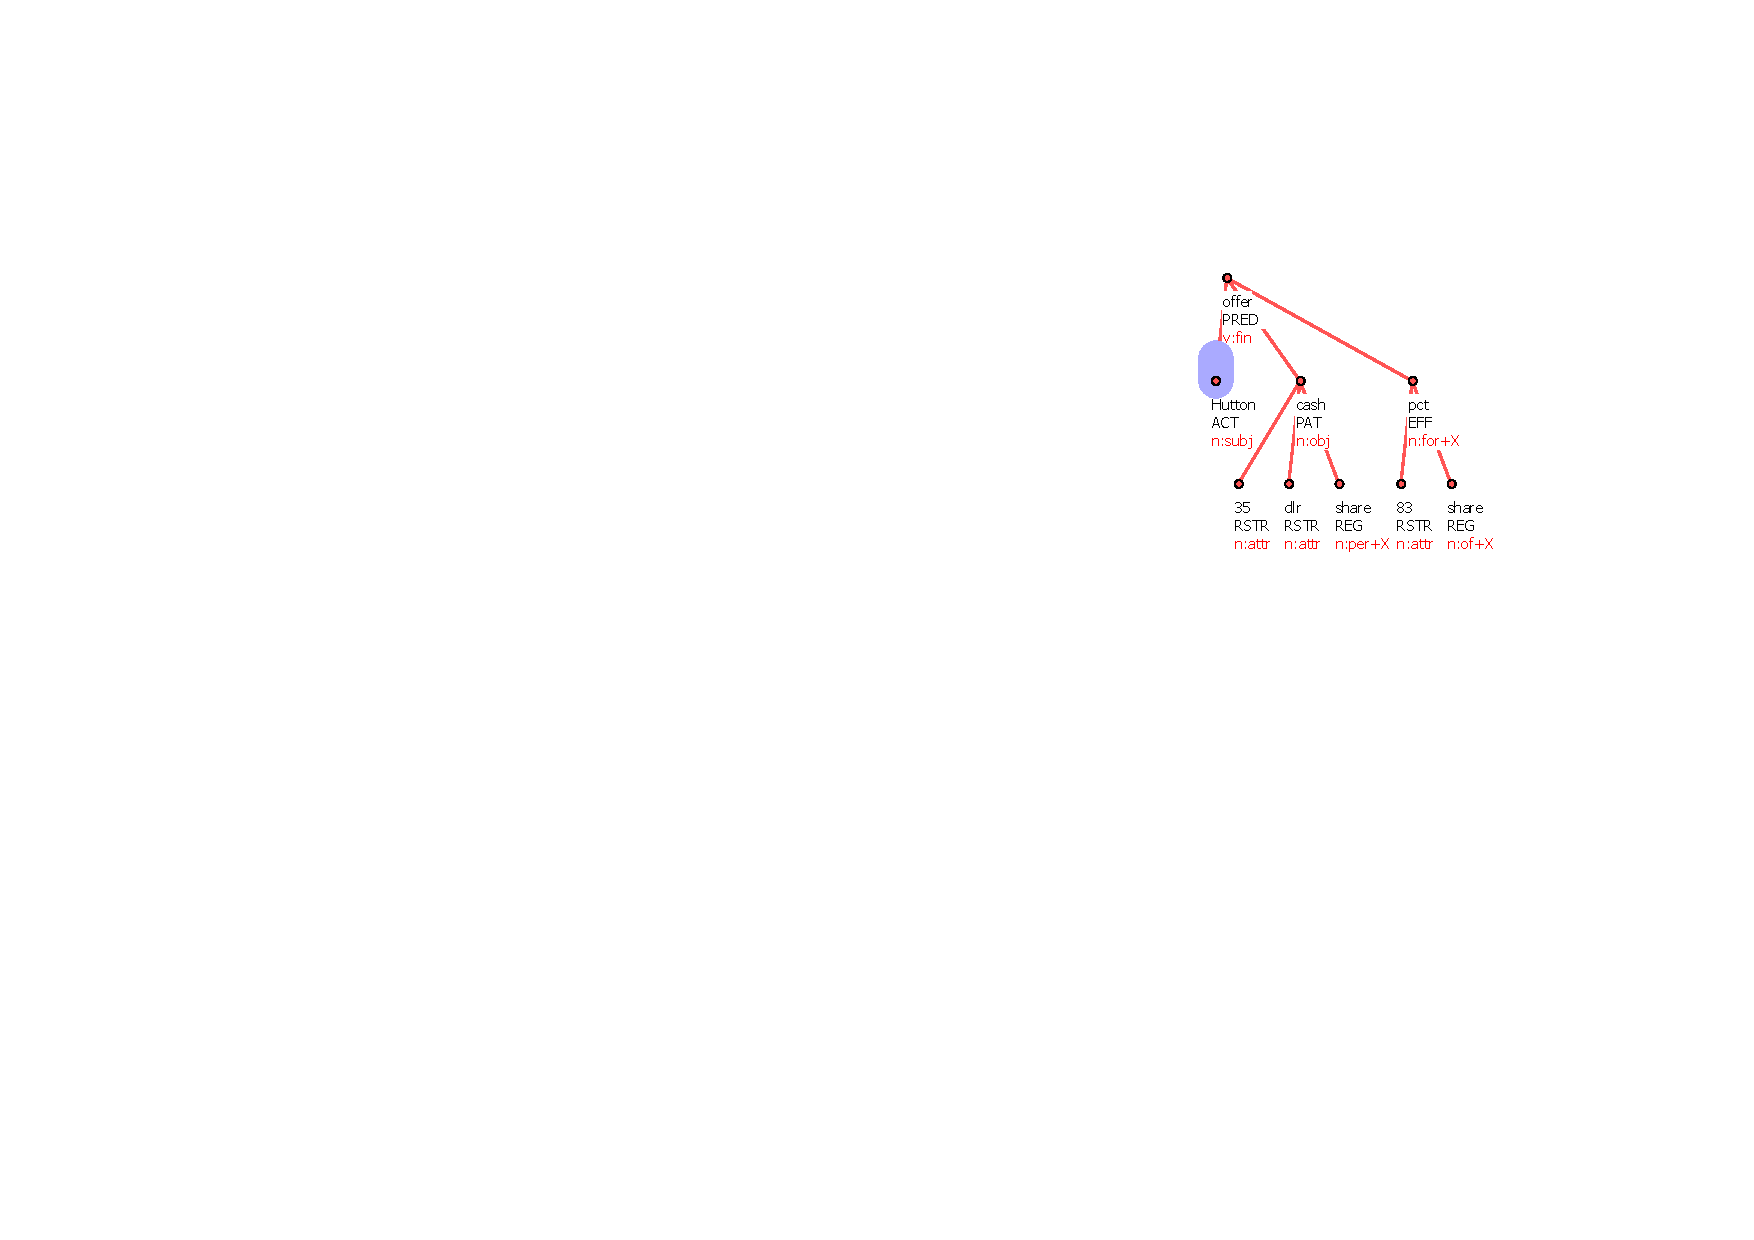
\includegraphics[width=0.5\hsize]{img/tree}}
\caption{Tectogrammatical tree of the sentence: ``Hutton is offering 35 dlrs cash per share for 83 pct of the shares.''
Nodes roughly correspond with words of a sentence, edges represent linguistic dependencies between nodes and some linguistic features (tectogrammatical lemma, semantic functor and semantic part of speech) are printed under each node. The node `Hutton' is docarated as a named entity.}
\label{img:tree}
\end{figure}



\subsubsection{Rule Transformations}

Extraction rules produced by the IE engine are natively kept in a Prolog format; examples can be seen in Fig.~\ref{img:rules_prolog}. The engine is capable to export them to the OWL/XML\footnote{\url{http://www.w3.org/TR/owl-xmlsyntax/}} syntax for rules in OWL 2 \cite{GHPP09a} (see in Fig.~\ref{img:rules_xml}). Such rules can be parsed by OWL API\footnote{\url{http://owlapi.sourceforge.net/}} 3.1. Fig.~\ref{img:rules_protege} shows the example rules in Prot\'{e}g\'{e} 4 -- Rules View's format. And the last rule example can be seen in Fig.~\ref{img:rules_jena}, which shows a rule in the Jena rules format \footnote{\url{http://jena.sourceforge.net/inference/#RULEsyntax}}. Conversion to Jena rules was necessary because it is the only format that Jena can parse, see details about our use of Jena in Section\ref{sec:experiment}. The Jena rules were obtained using following process: OWL/XML $\rightarrow$ RDF/SWRL\footnote{\url{http://www.w3.org/Submission/SWRL/}} conversion using OWL API and RDF/SWRL $\rightarrow$ Jena rules conversion using SweetRules\footnote{\url{http://sweetrules.semwebcentral.org/}}.



\begin{figure}
\small
[Rule 1] [Pos cover = 23 Neg cover = 6]\\
\verb@mention_root(acquired,A) :-@\\
\verb@   'lex.rf'(B,A), t_lemma(B,'Inc'), tDependency(C,B), tDependency(C,D),@\\
\verb@   formeme(D,'n:in+X'), tDependency(E,C).@
\smallskip\newline
[Rule 11] [Pos cover = 25 Neg cover = 6]\\
\verb@mention_root(acquired,A) :-@\\
\verb@   'lex.rf'(B,A), t_lemma(B,'Inc'), tDependency(C,B), formeme(C,'n:obj'), @\\
\verb@   tDependency(C,D), functor(D,'APP').@
\smallskip\newline
[Rule 75] [Pos cover = 14 Neg cover = 1]\\
\verb@mention_root(acquired,A) :-@\\
\verb@   'lex.rf'(B,A), t_lemma(B,'Inc'), functor(B,'APP'), tDependency(C,B), @\\
\verb@   number(C,pl).@
	\caption{Examples of extraction rules in the native Prolog format.}
	\label{img:rules_prolog}
\end{figure}

\begin{figure}
\small
[Rule 1]\\
\verb@lex.rf(?b, ?a), t_lemma(?b, "Inc"), tDependency(?c, ?b),@\\
\verb@tDependency(?c, ?d), formeme(?d, "n:in+X"), tDependency(?c, ?e)@\\
\verb@      -> mention_root(?a, "acquired")@
\smallskip\newline
[Rule 11]\\
\verb@lex.rf(?b, ?a), t_lemma(?b, "Inc"), tDependency(?c, ?b),@\\
\verb@formeme(?c, "n:obj"), tDependency(?c, ?d), functor(?d, "APP")@\\
\verb@      -> mention_root(?a, "acquired")@   
\smallskip\newline
[Rule 75]\\
\verb@lex.rf(?b, ?a), t_lemma(?b, "Inc"), functor(?b, "APP"),@\\
\verb@tDependency(?c, ?b), number(?c, "pl")@\\
\verb@      -> mention_root(?a, "acquired")@   
	\caption{Examples of extraction rules in Prot\'{e}g\'{e} 4 -- Rules View's format}
	\label{img:rules_protege}
\end{figure}

\begin{figure}[p]
\centerline{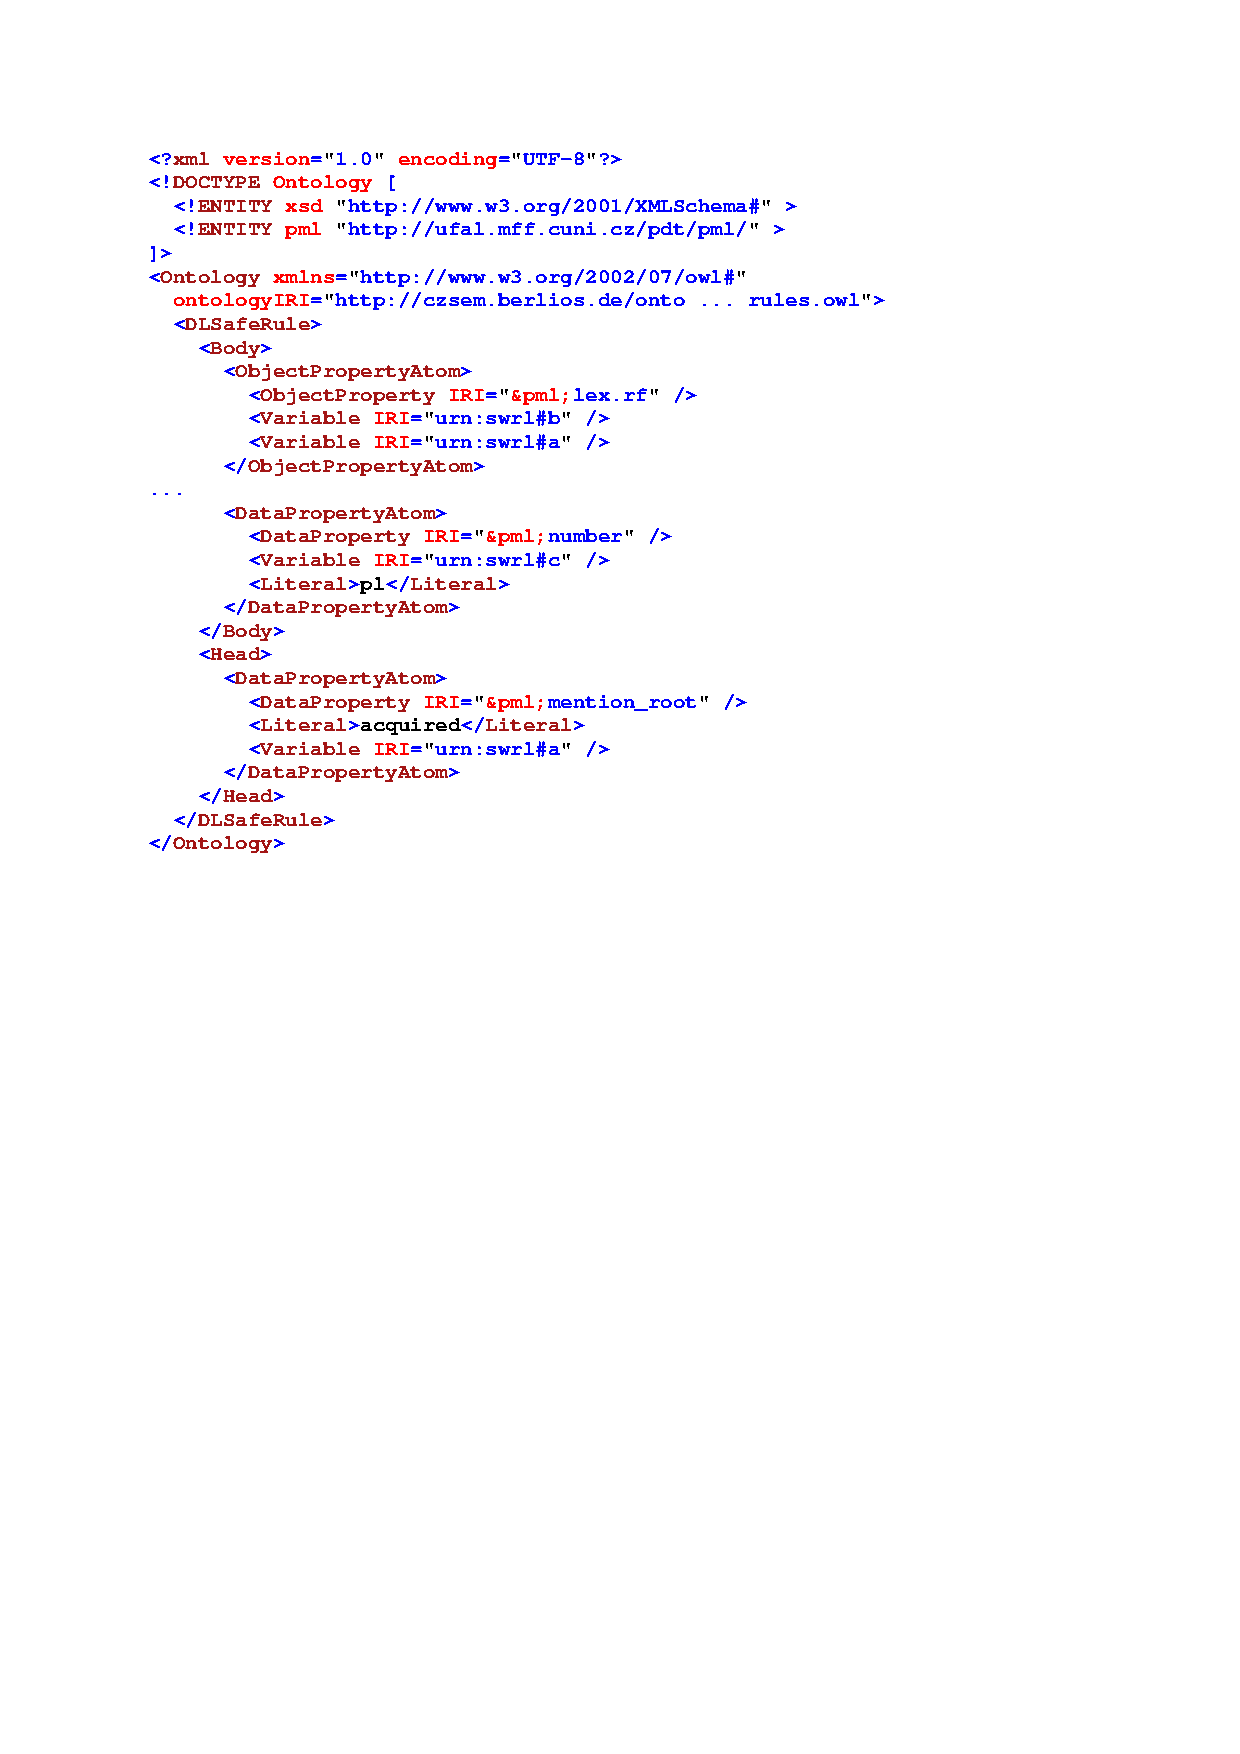
\includegraphics[width=0.9\hsize]{img/rules_owl_xml}}
\caption{Rule 75 in the OWL/XML syntax for Rules in OWL 2 \cite{GHPP09a}.}
\label{img:rules_xml}
\end{figure}


\begin{figure}[p]
\small
\begin{verbatim}
@prefix pml: <http://ufal.mff.cuni.cz/pdt/pml/>.
[rule-75:  
        ( ?b pml:lex.rf ?a )
        ( ?c pml:tDependency ?b )
        ( ?b pml:functor 'APP' )
        ( ?c pml:number 'pl' )
        ( ?b pml:t_lemma 'Inc' )
     -> 
        ( ?a pml:mention_root 'acquired' )
]
\end{verbatim}

\caption{Rule 75 in the Jena rules syntax.}
\label{img:rules_jena}
\end{figure}


\clearpage
\subsubsection{Schema of the Case Study}

Schema of the case study can be seen in Fig.~\ref{img:rules_app_schema}.  

The top row of the image illustrates how TectoMT (third party linguistic tool) linguistically annotates an input document and the linguistic annotations are translated to so-called document ontology by a GRDDL/XSLT transformation.

In the bottom of the picture our IE engine learns extraction rules and exports them to an extraction ontology. The reasoner in the middle is used to apply the extraction ontology on the document ontology and it produces the ``annotated'' document ontology, which was described in Section~\ref{sec:doc_ont}.


\begin{figure}
\centerline{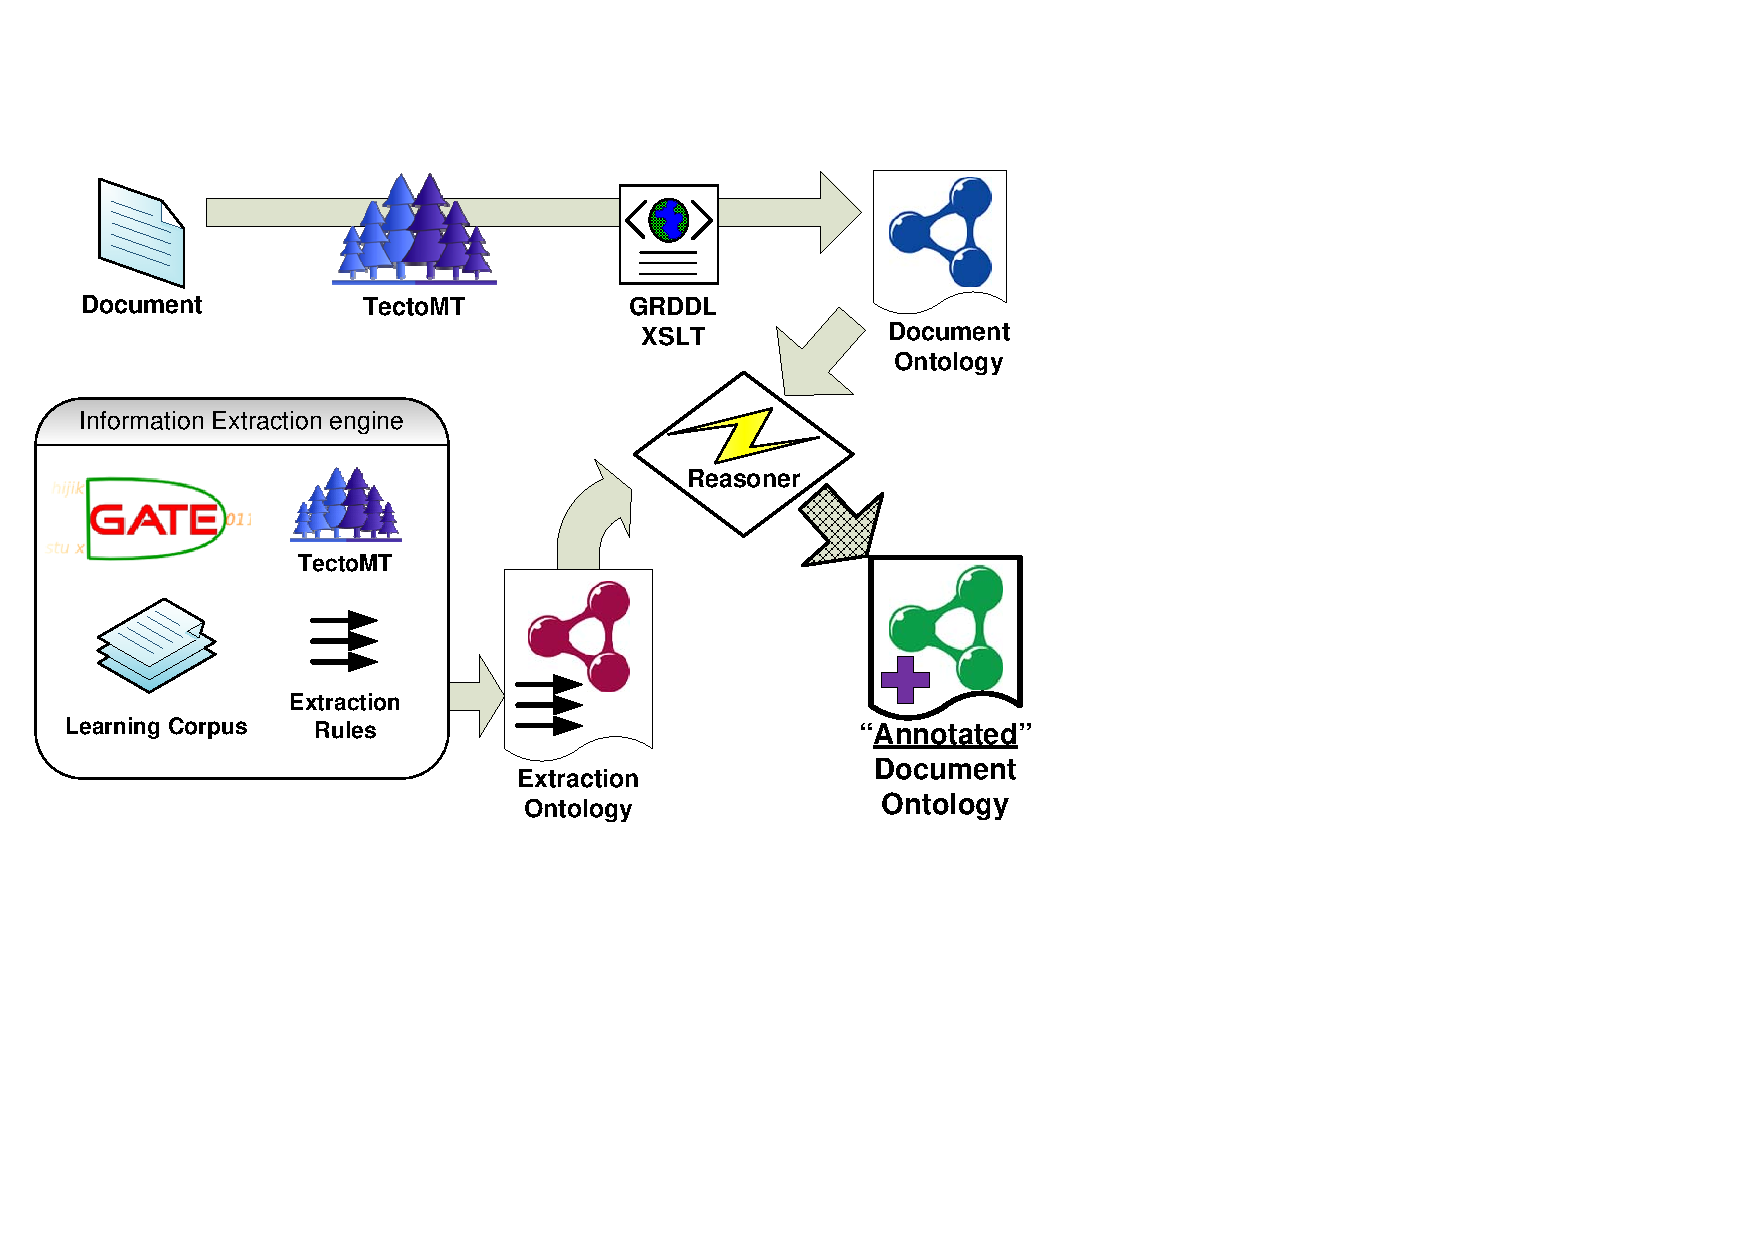
\includegraphics[width=\hsize]{img/semantic_rules_app_schema}}
\caption{Semantic annotation driven by an extraction ontology and a reasoner -- schema of the process.}
\label{img:rules_app_schema}
\end{figure}


\subsubsection{How to Download}
All the resources (including source codes of the case study and the experiment) mentioned in this demonstration are publically available on the web-page of our project\footnote{\url{http://czsem.berlios.de/}} and detailed information can be found there.


%%%%%%%%%%%%%%%%%%%%%%%%%%%%%%%%%%%%%%%%%%%%%%%%%%%%%%%%%%%%%%%%%%%%%%%%%%%%%%%%%%%%%%%%%%%%%%%%%%%%%%%%%%%%%%
\section{Experiment} \label{sec:experiment}
%%%%%%%%%%%%%%%%%%%%%%%%%%%%%%%%%%%%%%%%%%%%%%%%%%%%%%%%%%%%%%%%%%%%%%%%%%%%%%%%%%%%%%%%%%%%%%%%%%%%%%%%%%%%%%


In this section we present an experiment that should serve as a proof of a concept that the proposed idea of independent extraction ontologies is working. We have selected several reasoners (namely Jena, HermiT, Pellet and FaCT++) and tested them on two slightly different datasets from two different domains and languages (see Table~\ref{tab:datasets}). This should at least partially demonstrate the universality of the proposed approach.

In both cases the task is to find all instances (corresponding to words in a document) that should be uncovered by the extraction rules. The extraction rules are saved in single extraction ontology for each dataset. The datasets are divided into individual document ontologies (owl files) corresponding to the individual documents of a source IE dataset (see below). During an experiment the individual document ontologies are processed separately (one ontology in a step) by a selected reasoner. The total time taken to process all document ontologies of a dataset is the measured result of the experiment. 

The actual reasoning task is more difficult than a simple retrieval of all facts entailed by the extraction rules. Such simple retrieval task took only a few seconds for the Acquisitions v1.1 dataset (including parsing) in the native Prolog environment that the IE engine uses. There were several more inferences needed in the reasoning task because the schema of the input files was a little bit different form the schema used in rules. The mapping of the schemas was captured in another ontology that was included in the reasoning task. The mapping ontology is a part of the publically available project ontologies \footnote{See ``Data $\rightarrow$ ontologies'' link on the project page \url{http://czsem.berlios.de/}} and a potentially interested reader can find the complete mapping there.


\subsection{Datasets}

In the experiment we used two slightly different datasets from two different domains and languages.  Table~\ref{tab:datasets} summarizes some basic information about them.

\begin{table}
\begin{tabular}{|r||r|r|c|r|c|}
\hline
dataset & domain & language & number of files & dataset size & number of rules\\
\hline
\hline
czech\_fireman & accidents & Czech & 50 & 16 MB & 2\\
\hline
acquisitions-v1.1 & finance & English & 600 & 126 MB & 113\\
\hline
\end{tabular}
\caption{Description of datasets that we have used.}
\label{tab:datasets}
\end{table}


\subsubsection{czech\_fireman}


The fist dataset is called `czech\_fireman'. This dataset was created by ourselves during the development of our IE  engine. It is a collection of 50 Czech texts that are reporting on some accidents (car accidents and other actions of fire rescue services). These reports come from the web of Fire rescue service of Czech Republic\footnote{\url{http://www.hzscr.cz/hasicien/}}. The labeled corpus is publically available on the web of our project\footnote{\url{http://czsem.berlios.de/}}.
The corpus is structured such that each document represents one event (accident) and several attributes of the accident are marked in text. For the experiment we selected the `damage' task -- to find an amount (in CZK - Czech Crowns) of summarized damage arisen during a reported accident.





\subsubsection{Acquisitions v1.1}  

The second dataset is called ``Corporate Acquisition Events'' corpus and it is
described in \cite{lewis1992representation}. More precisely we use the \emph{Acquisitions v1.1} version\footnote{This version of the corpus comes form the Dot.kom (Designing infOrmation extracTion for KnOwledge Management) project's resources: \url{http://nlp.shef.ac.uk/dot.kom/resources.html}} of the corpus.
This is a collection of 600 news articles describing acquisition
events taken from the Reuters dataset. News articles are tagged to identify fields
related to acquisition events. These fields include `purchaser' , `acquired', and
`seller' companies along with their abbreviated names (`purchabr', `acqabr' and
`sellerabr') Some news articles also mention the field `deal amount'.
For the experiment we selected only the `acquired' task.





\subsection{Reasoners}

In the experiment we used four OWL reasoners (namely
Jena\footnote{\url{http://jena.sourceforge.net}}
,HermiT\footnote{\url{http://hermit-reasoner.com}}
,Pellet\footnote{\url{http://clarkparsia.com/pellet}}
and FaCT++\footnote{\url{http://code.google.com/p/factplusplus}}
) and measured the time they needed to complete a particular task. The time also includes time spend on parsing the input. HermiT, Pellet and FaCT++ were called through OWLAPI-3.1, so the same parser was used for them. Jena reasoner was used in its native environment and used the Jena parser.

In the early beginning of the experiment we had to exclude the FaCT++ reasoner form all tasks. It tuned out that FaCT++ probably does not work with rules in our setting (We called FaCT++ through OWLAPI-3.1) because it does not returned any result instances.  All the remaining reasoners strictly agreed on the results and returned the same sets of instances.

Also HermiT was not fully evaluated on the Acquisitions v1.1 dataset because it was too slow. The reasoner spent 13 hours of running to process only 30 of 600 files of the dataset. And we did not find it useful to let it continue.




%\subsection{HermiT experiment}

%After 13 hours of reasoning only 30 files (of 600) were processed.














\subsection{Evaluation Results of the Experiment}






\begin{table}
\begin{center}
\begin{tabular}{|r||r|r||r|r|}
\hline
reasoner & \textbf{czech\_fireman} & stdev & \textbf{acquisitions-v1.1} & stdev\\
\hline
\hline
Jena & 161 s & 0.226 & 1259 s & 3.579\\
\hline
HermiT & 219 s & 1.636 & $\gg$ 13 hours & \\
\hline
Pellet & 11 s & 0.062 & 503 s & 4.145\\
\hline
FaCT++ & \multicolumn{4}{|c|}{Did not work with rules in our setting.}\\
\hline
\end{tabular}
\end{center}
\caption{Time performance of tested reasoners on both datasets. Time is measured in seconds. Average values from 6 measurements. Experiment environment: Intel Core I7-920 CPU 2.67GHz, 3GB of RAM, Java SE 1.6.0\_03, Windows XP.}
\label{tab:results}
\end{table}

Table\ref{tab:results} summarizes results of the experiment. The standard deviations are relatively small when compared to the differences between the average times.  So there is no doubt about the order of the tested reasoners. Pellet performed the best and HermiT was the slowest amongst the tested and usable reasoners in this experiment.

From the results we can conclude that similar tasks can be satisfactorily solved by contemporary reasoners because three of four tested reasoners were working in the presented tasks and two reasoners finished in operational time.






\subsection{Repeatability}

Our implementation is publicly available -- source codes and the datasets can be downloaded from our project's web-page\footnote{\url{http://czsem.berlios.de/}}, so the experiment should be repeatable according to the SIGMOD Experimental Repeatability Requirements \cite{biblio:SIGMODrepeatability}.

\section{Future Work}

Annotated document ontology $\rightarrow$ fact ontology

\section{Conclusion}

\bigskip
\noindent\textbf{Acknowledgments}\\
This work was partially supported by Czech projects: GACR P202/10/0761, GACR-201/09/H057, GAUK 31009 and MSM-0021620838.





\bibliographystyle{splncs03}
\bibliography{DedekVojtas_ESWC2010_semantically}
\end{document}
